\documentclass[12pt]{article}

\usepackage{ucs}
\usepackage[utf8x]{inputenc} % Включаем поддержку UTF8
\usepackage[russian]{babel}  % Включаем пакет для поддержки русского языка
\usepackage[left=2cm,right=2cm,top=2cm,bottom=2cm,bindingoffset=0cm]{geometry}
\usepackage[pdftex]{graphicx, color}
\usepackage{subfigure}
\usepackage{color}
\usepackage{listings}
\usepackage{multirow}

\usepackage{algorithm}
\usepackage{algorithmicx}
\usepackage{algpseudocode} 

\algnotext{EndFor} 
\algnotext{EndIf} 
\algrenewcommand\algorithmicrequire{\textbf{Precondition:}} 
\algrenewcommand\algorithmicensure{\textbf{Postcondition:}} 
\newcommand*\Let[2]{\State #1 $\gets$ #2} 
\renewcommand{\algorithmiccomment}[1]{\hskip2em$\triangleright$ #1}

\usepackage[nooneline]{caption} \captionsetup[table]{justification=raggedleft} \captionsetup[figure]{justification=centering,labelsep=endash}

\renewcommand{\baselinestretch}{1.5}

\lstset{inputencoding=utf8x, extendedchars=false, keepspaces = true,
   language=c}
\renewcommand{\lstlistingname}{Листинг}

\RequirePackage{enumitem}
\renewcommand{\alph}[1]{\asbuk{#1}}
\setlist{nolistsep}
\setitemize[1]{label=---, fullwidth, itemindent=\parindent, 
  listparindent=\parindent}
\setitemize[2]{label=---, leftmargin=2cm} % для дефисного списка

\usepackage{amsmath}
\usepackage{amssymb}
\usepackage{pifont}

\usepackage{float}
\floatname{algorithm}{Листинг}

\newcommand{\subsetmin}{\underset{\scriptscriptstyle\min}{\subset}}
\newcommand{\minsubset}{\subsetmin}

\begin{document} % начало документа

\setcounter{tocdepth}{4} % chapter, section, subsection, subsubsection и paragraph

\graphicspath{{chapter1/},{chapter3/}}
\DeclareGraphicsExtensions{.png,.pdf,.jpg,.mps,.xfc}

\renewcommand{\contentsname}{\centering Содержание}
\parindent = 0.7cm

\begin{titlepage} % начало титульной страницы

\begin{center} % включить выравнивание по центру

\textit {Государственное образовательное учреждение высшего профессионального образования}\\

\huge«Московский государственный технический университет имени Н.Э. Баумана»\\
\Large {(МГТУ им. Н.Э. Баумана)}\\[0.2cm] 

\rule[+3mm]{7.5cm}{0.80mm}

\end{center} 

\begin{flushleft} % выровнять содержимое по левому краю


\begin{tabbing}
MMMMММММMМ \= \kill
\large{ФАКУЛЬТЕТ} \> \large{\textit{ИНФОРМАТИКА И СИСТЕМЫ УПРАВЛЕНИЯ}} \\
\large{КАФЕДРА} \> \large{\textit{ТЕОРЕТИЧЕСКАЯ ИНФОРМАТИКА}} \\
 \> \large{\textit{И КОМПЬЮТЕРНЫЕ ТЕХНОЛОГИИ}}
\\
\end{tabbing}


\end{flushleft} 

\begin{center}


\Huge{РАСЧЕТНО-ПОЯСНИТЕЛЬНАЯ ЗАПИСКА}\\
к курсовому проекту на тему:\\
Оптимизация образцовых выражений в языке программирования РЕФАЛ\\[1.0cm]


\begin{tabbing}
MMMMММММMMMMMMMMMM \= \kill
\Large{Студент} \> \Large{\textit{Батусов П. В.}} \\
\Large{Руководитель курсового проекта} \> \Large{\textit{Коновалов А. В.}}\\[0.5cm]
\end{tabbing}

\largeМосква 2014

\end{center}

\thispagestyle{empty} % не нумеровать страницу
\end{titlepage} % конец титульной страницы

\renewcommand{\abstractname}{\Huge{Аннотация\\[1.5cm]}}

\begin{abstract}
В данной работе рассматриваются возможные методы и подходы для оптимизации образцовых выражений в языке программирования РЕФАЛ. Цель поставленной задачи --- доработка компилятора, порождающего более быструю исполняемую программу. В работе описывается и обосновывается необходимость данной оптимизации, а также производится оценка производительности оптимизированных программ.
\end{abstract}

\clearpage
\tableofcontents %Содержание
\newpage

\part*{\large \centering ВВЕДЕНИЕ}
\addcontentsline{toc}{part}{ВВЕДЕНИЕ}
\hspace{\parindent}РЕФАЛ --- РЕкурсивных Функций АЛгоритмический язык программирования, является одним из старейших функциональных языков, ориентированный на символьные вычисления: обработку символьных строк (например, алгебраические выкладки); перевод с одного языка (искусственного или естественного) на другой; решение проблем, связанных с искусственным интеллектом. Соединяет в себе математическую простоту с практической ориентацией на написание больших и сложных программ \cite{RefalOverview}. \\
\indent Первая версия РЕФАЛа была создана в 1966 году Валентином Турчиным в качестве метаязыка для описания семантики других языков. Впоследствии, в результате появления достаточно эффективных реализаций на ЭВМ, он стал находить практическое использование в качестве языка программирования \cite{RefalHistory}. \\
\indent РЕФАЛ программа может состоять из одного или нескольких модулей (файлов), каждый из которых, в свою очередь, состоит из функций. РЕФАЛ-функция представляет собой упорядоченный набор предложений, состоящих из образца и шаблона. На вход функции подается некоторое выражение; вычисление функции состоит в сопоставлении выражения поочередно образцам, взятым из первого, второго и т. д. предложений. Если очередное сопоставление проходит успешно, то на основании шаблона, взятого из того же предложения, формируется новое РЕФАЛ-выражение, которое и будет результатом функции. В случае, если ни с одним из имеющихся образцов аргумент функции сопоставить не удалось, фиксируется ошибка (аварийно завершается вся программа). Во избежание этого часто в конце функции помещают предложение, с образцом которого можно сопоставить вообще произвольное выражение. В некоторых современных реализациях РЕФАЛа (например, РЕФАЛ+) неуспех любого выражения функции вместо ошибки порождает неуспех самой функции. \\
\indent В РЕФАЛе, как и во многих других функциональных языках программирования, в отличие от императивных языков, отсутствуют циклы. Для описания циклических процессов используется рекурсия. Зачастую, при таком подходе, тело функции, реализующей цикл, содержит большое число предложений, с очень похожими образцами. Если оптимизировать их вычисление, например создать дерево из левых частей предложений (в пределах одной функции), чтобы операторы, общие для нескольких предложений, выполнялись только один раз, это может дать большой прирост скорости выполнения программы.

\newpage

\section[Базисный РЕФАЛ]{\large \centering Базисный РЕФАЛ}
\hspace{\parindent}РЕФАЛ является одним из старейших функциональных языков, отличительная черта которого --- использование сопоставления с образцом и переписывания термов как основного способа определения функций.

\subsection[Предложения и функции]{\large Предложения и функции}
\hspace{\parindent}Предложением называется конструкция вида: <<образцовое выражение = результатное выражение;>>. Образец часто называют левой частью, результат --- правой частью, в которой могут использоваться только те переменные, которые определены в левой части.\\ \indent РЕФАЛ-функция представляет собой упорядоченный набор таких предложений. Ее выполнение заключается в сопоставлении переданного аргумента с левой частью первого предложения. Если сопоставление оказывается успешным, то значения переменных, определенных в образце, подставляются в правую часть и вызов функции заменяется на получившийся результат. При неудачном сопоставлении с образцом, точно таким же образом выполняется второе предложение и т. д. Если сопоставление не удалось в левой части последнего предложения, то программа прекращает работу с ошибкой невозможности сопоставления (recognition impossible).\\
\indent Обычно в левых частях выражений рассматриваются различные варианты допустимых аргументов, поэтому ошибка невозможности сопоставления часто говорит о том, что или на вход функции был передан некорректный аргумент, или сама функция написана с ошибкой. Таким образом, в РЕФАЛ четко разделены операции анализа аргумента, выполняемые при помощи сопоставления с образцом, и операции синтеза, осуществляемые при помощи подстановки значений переменных в результатное выражение. \\
\indent В качестве аргументов функции передается последовательность (возможно пустая) термов, которыми могут быть:

\begin{itemize}
\item обыкновенные символы --- буквы, цифры и т. д.;
\item символы-метки (идентификаторы);
\item цифры --- цифровая запись неотрицательных целых чисел, не превышающих предельное значение;
\item выражение в структурных скобках;
\item активное выражение (означающее вызов функции);
\end{itemize}

\subsection[Сопоставление с образцом]{\large Сопоставление с образцом}
\hspace{\parindent}Образцы РЕФАЛа могут содержать свободные переменные, которые состоят из указателя типа, точки и индекса. Индексом переменной является последовательность букв и цифр. Есть три указателя типа. Они обозначаются малыми буквами s, t и e, а соответствующие им переменные называются  s-, t- и e-переменными. Различие между ними состоит в множествах их допустимых значений.  Значением s-переменной может служит только один символ, а t-переменной --- любой терм. Значением e-переменной может быть любое выражение~\cite{RefalBasis}. \\
\indent Если в образце присутствует несколько вхождений переменных с одинаковым типом и одинаковым именем, то такие переменные называются повторными. Все вхождения повторной переменной должны иметь одинаковое значение. В образце не может быть переменных, имеющих одинаковое имя, но при этом разные типы.\\
\indent Сопоставлением объектного выражения E с образцом P называется поиск значений переменных, входящих в образец P, подстановка которых в P дает выражение E. Если такие значения найти невозможно, то сопоставление считается неуспешным. \\
\indent Если существует несколько вариантов сопоставления, то выбирается тот, в котором первая переменная (при чтении слева-направо) принимает кратчайшее значение (имеется ввиду длина в термах). Если это правило не устраняет неоднозначности, то анализируется следующая переменная и т. д. При таком соглашении сопоставление в РЕФАЛе становится однозначной операцией. \\
\indent Для разных образцовых выражений операция сопоставления будет выполняться за разное время. Так, например простые операции: сопоставление с атомом, s-переменной, с парой скобок выполняются за постоянное время, а сопоставления каждой открытой e-переменной линейно зависит от длины <<сканируемого>> объектного выражения, поэтому одна e-переменная добавляет линейную сложность, две — квадратичную, три — кубическую. Повторная t- или e-переменная требует рекурсивного сравнения объектных термов или объектных выражений, соответственно, поэтому сложность сопоставления линейно зависит от числа атомов и скобок, входящих в сравниваемые выражения. Пара повторных переменных требует одного сравнения, 3 переменных — двух сравнений и т. д.

\subsection[Необходимость оптимизации]{\large Необходимость оптимизации}
\hspace{\parindent} Синтаксис РЕФАЛа не позволяет функциям принимать более одного аргумента --- объектного выражения. При передачи нескольких параметров, они <<склеиваются>> в одно объектное выражение, которое потом в теле функции приходится разбирать на части соответствующие входным аргументам. Таким образом зачастую можно встретить ситуацию, когда несколько образцовых частей предложения одной функции имеют похожую структуру, в результате чего одни и те же операции анализа аргумента функции выполняются несколько раз. Это крайне неэффективно, особенно если такая функция описывает некоторый циклический процесс. Кроме этого, оптимизация необходима в случае если компилятор РЕФАЛа порождает код для каждого предложения функции отдельно (пример --- рис. \ref{fig:code_gen}).

\begin{figure}[h!]
\centering
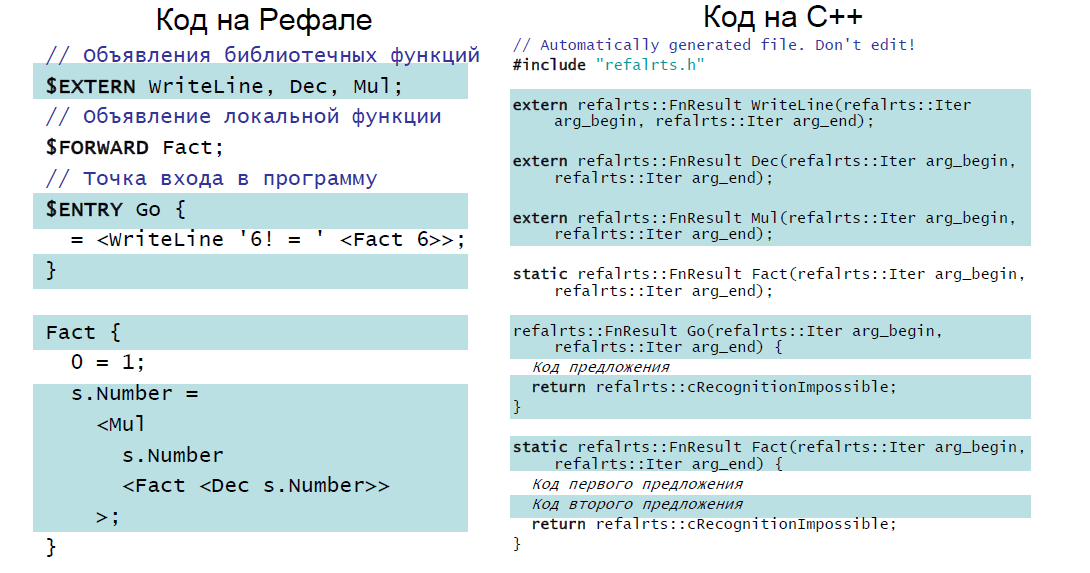
\includegraphics[width=1\linewidth]{./chapter1/code_gen}
\caption{Генерация кода в простом РЕФАЛе}
\label{fig:code_gen}
\end{figure}


\subsection[Постановка задачи]{\large Постановка задачи}
\hspace{\parindent}Задачей данного курсового проекта является разработка алгоритма оптимизации, устраняющего избыточность операции анализа аргумента функции для предложений, имеющих похожую структуру образцовых частей.

\newpage

\section[Алгоритм оптимизации]{\large \centering Алгоритм оптимизации}
\hspace{\parindent}Одним из возможных методов удаления избыточных сопоставлений с образцом является обобщение левых частей подряд идущих предложений. 
\subsection[Жесткий образец]{\large Жесткий образец}
\hspace{\parindent} Введем некоторые определения. \textit{Объектное выражение} (или, для краткости, просто <<выражение>>)~---~это последовательность из термов, каждый из которых может быть либо атомарным, либо скобочным термом, т.е. выражением, заключенным в круглые скобки. \textit{Атомарные термы} (атомы) --- это термы, которые невозможно разбить на составные части путем сопоставления с образцом, обычно к ним относятся атомы-числа, атомы-символы, атомы-имена и т.д. Будем обозначать атомы как \(X_1, X_2, \dots, X_n\). Сами объектные выражения будем обозначать латинской буквой \(E\), иногда с индексом.\\
\indent \textit{Образцовое выражение} (образец) --- это синтаксическая конструкция, позволяющая описать некоторое множество объектных выражений. Оно записывается как объектное выражение, но некоторые части заменяются особыми подстановочными знаками --- переменными. Переменная может заменять либо любой атом (так называемая s"=переменная), либо любой терм (t"=переменная), либо некоторый правильный (с правильной расстановкой скобок) фрагмент выражения (e"=переменная). Переменные могут иметь имена для ссылок на них из результатных выражений, либо для указания того факта, что две одноименные переменные (они должны быть одного типа) заменяют одну и ту же часть объектного выражения.\\
\indent \textit{Жесткий образец} --- выражение без открытых и повторных переменных. Таким образом жесткое выражение на каждом уровне скобок содержит не более чем одну e-переменную, а индексы всех переменных, входящих в одно и то же жесткое выражение, должны быть попарно различны. Таким образом, жесткие образцы имеют следующий вид:\\

Образец := Терм* [e"=переменная Терм*].

Терм := Атом | t"=переменная | s"=переменная | (Образец).

Атом := X | s"=переменная.

\subsection[Уточнение образцов]{\large Уточнение образцов}
\hspace{\parindent} \textit{Подстановка} --- замкнутая на множестве жестких образцов замена переменных в образце соответствующими образцами ($S = \{ e_1 \to p_1, t_2 \to p_2, \ldots \} $ $ P \xrightarrow{S} P^{'} $). Один из возможных примеров подстановки (\ref{eq:math:insert_example}). 
\begin{equation}\label{eq:math:insert_example}
\begin{array}{l l l}
P & = & t_1 e_2 t_3 \\
S & = & \{ t_1 \to (e_4), e_2 \to s_5 e_6 \} \\
P^{'} & = & (e_4) s_5 e_6 t_3
\end{array}
\end{equation} 

\indent Если один образец \(P_1\) можно получить из другого образца \(P_2\) подстановкой, то будем говорить, что \(P_1\) \textit{уточняет} \(P_2\), а \(P_2\), соответственно, \textit{обобщает} \(P_1\).  Введем следующие обозначения для операции уточнения образцов:

\(P_1 \Rightarrow^+ P_2\) --- $P_1$ уточняет $P_2$

\(P_1 \Rightarrow^* P_2\) --- нестрогое уточнение, $P_1 \Rightarrow^+ P_2$ или $P_1 = P_2$

\indent Не трудно догадаться, что e обобщает любой образец: $\forall P e \Rightarrow^* P$.\\
\indent Пусть \(P_1 \Rightarrow^+ P_2\), и при этом не существует такого образца \(P_3\), что \(P_1 \Rightarrow^+ P_3 \Rightarrow^+ P_2\). Тогда \(P_1\) будем называть \textit{минимальным уточнением} \(P_2\) (и, соответственно, \(P_2\) --- \textit{минимальным обобщением} \(P_1\)) и обозначать как \(P_1 \underset{\scriptscriptstyle\min}{\Rightarrow} P_2\).\\
\indent Заметим, что \(P_1 \underset{\scriptscriptstyle\min}{\Rightarrow} P_2\) тогда и только тогда, когда \(P_1\) можно получить из \(P_2\) только одной из следующих замен:
\begin{equation}\label{eq:math:simpletransform}
\begin{array}{l l l}
e & \to & te \\
e & \to & et \\
t & \to & (e) \\
t & \to & s \\
s & \to & X
\end{array}
\end{equation}

Если \(P \Rightarrow^+ Q\) и можно построить цепочку минимальных уточнений от \(Q\) до \(P\) двумя способами, т.\,е.
\begin{equation*}
\begin{array}{l}
P \underset{\scriptscriptstyle\min}{\Rightarrow} R_1 \underset{\scriptscriptstyle\min}{\Rightarrow} R_2 \underset{\scriptscriptstyle\min}{\Rightarrow} \ldots \underset{\scriptscriptstyle\min}{\Rightarrow} R_n \underset{\scriptscriptstyle\min}{\Rightarrow} Q \\
P \underset{\scriptscriptstyle\min}{\Rightarrow} R'_1 \underset{\scriptscriptstyle\min}{\Rightarrow} R'_2 \underset{\scriptscriptstyle\min}{\Rightarrow} \ldots \underset{\scriptscriptstyle\min}{\Rightarrow} R'_m \underset{\scriptscriptstyle\min}{\Rightarrow} Q
\end{array}
\end{equation*}
то \(n = m\).

Чтобы это показать, ведём числовую характеристику образца \(C(P)\), которую определим как
\begin{equation*}
C(P) = n_t + 2n_s + 3n_X + 3n_{()} - n_e + 1
\end{equation*}
Здесь \(n_t\), \(n_s\), \(n_e\) --- число, соответственно t"=переменных, s"=переменных, e"=переменных, \(n_{()}\) --- число пар круглых  скобок, \(n_X\) "--- число литералов атомов. Нетрудно убедиться, что для каждого преобразования \eqref{eq:math:simpletransform} величина \(C(P)\) возрастает на~1, следовательно, минимальное уточнение увеличивает данную величину на~1. Поскольку \(C(P)\) и~\(C(Q)\) зависят только от внешнего вида образца, число элементарных уточнений между \(P\) и~\(Q\) не~будет зависеть от~<<траектории>> перехода. Определим \textit{сложность сопоставления} для образца P как число минимальных уточнений от $e$ до $P$ --- $C(P)$. Заметим, что $C(e) = 0$.

\subsection[Обобщение образцов]{\large Обобщение образцов}
\hspace{\parindent} Рассмотрим множество образцов $P_1 \ldots P_N$. Будем называть \textit{глобальным сложнейшим обобщением (ГСО)} такое $P^*\Rightarrow^*P_i, i = 1 \ldots N$, что $\nexists Q \Rightarrow^* P_i,$ $C(Q) > C(P^*)$. Аналогичным образом определим \textit{локально сложнейшее обобщение (ЛСО)} $P^*\Rightarrow^+ Q$. Заметим, что ГСО($P_1 \ldots P_N$) $\subseteq$ ЛСО($P_1 \ldots P_N$). Ниже (\ref{eq:math:lso_gso_example}), представлен пример ЛСО и ГСО дл двух образцов $P_1 = stt$ и $P_2 = st$.
\begin{equation}\label{eq:math:lso_gso_example}
\begin{array}{l}
\textrm{ЛСО}(stt, st) = \{ste, set, ett\} \\
\textrm{ГСО}(stt, st) = \{ste, set\} \\
e_1 t_2 t_3 \xrightarrow{e_1 \to s} s t_2 t_3 \\
e_1 t_2 t_3 \xrightarrow{e_1 \to \varepsilon, t_2 \to s} s t_3
\end{array}
\end{equation} 
\indent Пусть $S_1 \ldots S_N$ --- подстановки переменных $v_1 \ldots v_k$, $S_i = \{v_j \rightarrow P_{ij}\}$, где P --- это некоторый образец с этими переменными. Обозначим за $P_i$ подстановку $S_i$ в образец $P$. Если $P \xrightarrow{S^*} P^* ,$ где $S^* = \{v_j \rightarrow P^*_j\}$, то $P^* \in$ ЛСО($P_1 \ldots P_N$) тогда и только тогда, когда $P^*_j \in$ ЛСО($P_{1j} \ldots P_{Nj}$). Аналогично верно и для ГСО.\\
\indent Определим \textit{быстрое обобщение (БО)} для двух образцов $P_1$ и $P_2$ следующим образом:\\
\indent 1) если $P_1$ и $P_2$ являются термами, то БО определется согласно таблице \ref{tab:bo}.
\begin{table}[h]
\caption{\label{tab:bo}Правила быстрого обобщения для двух термов}
\begin{center}
\begin{tabular}{|c|c|c|c|c|}
\hline
\multirow{2}{*}{$P_1$}   & \multicolumn{4}{c|}{$P_2$}                                                                                                 \\ \cline{2-5} 
                        & x & s & ($P_2^{'}$) & t \\ \hline
x & x & s & t & t \\ \hline
y $\neq$ x & s & s & t & t \\ \hline
s & s & s & t & t \\ \hline
($P_1^{'}$) & t & t & (БО($P_1^{'}$, $P_2^{'}$)) & t \\ \hline
t & t & t & t & t \\ \hline
\end{tabular}
\end{center}
\end{table}\\
\indent 2) Если $P_1$ и $P_2$ имеют следующий вид:
\begin{equation*}
P_1 = L_1^1 \ldots L_{M_1}^1 e R_{N_1}^1 \ldots R_1^1 
\end{equation*}
\begin{equation*}
P_2 = L_1^2 \ldots L_{M_2}^2 e R_{N_2}^2 \ldots R_1^2
\end{equation*}
\indent то БО($P_1, P_2$) = $L_1^* \ldots L_{min(M_1,M_2)}^* e R_{min(N_1,N_2)}^* \ldots R_1^*$, где $L_i^* = $ БО($L_i^1,L_i^2$), $R_i^* = $ БО($R_i^1,R_i^2$). \\
\\
\\
\indent 3) Если $P_1$ и $P_2$ имеют вид:
\begin{equation*}
P_1 = T_1^1 \ldots T_k^1 
\end{equation*}
\begin{equation*}
P_2 = T_1^2 \ldots T_k^2
\end{equation*}
\indent то БО($P_1, P_2$) = $T_1^* \ldots T_k^*$, где $T_i^* = $ БО($T_i^1,T_i^2$).\\
\indent 4) Во всех остальных случаях БО$ = e$.\\
\indent Заметим следующие свойства быстрого обобщения образцов:
\begin{itemize}
\item сложность алгоритма $O(len(P_1)+len(P_2))$, где $len(P)$ --- длинна образца образца $P$
\item БО($P_1$, БО($P_2, P_3$)) = БО(БО($P_1$, $P_2$), $P_3$)
\end{itemize}

\indent Определим БО($P_1 \ldots P_N$) как БО(БО($P_1 \ldots P_{N-1}$), $P_N$). \\
\indent БО($P_1 \ldots P_N$) $\Rightarrow^*$ ЛСО($P_1 \ldots P_N$)

\subsection[Сложнейший жесткий образец]{\large Сложнейший жесткий образец} \label{sec:sjo}
\hspace{\parindent} Обозначим $\mathbb{P}$ --- множество всех образцов, $\mathbb{H}$ --- множество жестких образцов. \textit{Сложнейший жесткий образец (СЖО)} $P_H \in \mathbb{H}$ для образца $P \in \mathbb{P}$ --- это такой образец, что $P \Rightarrow^* P_H$ и $\nexists P_H^{'} \in \mathbb{H}$ $ P \Rightarrow^* P_H^{'}$, $C(P_H^{'}) > C(P_H)$. На листинге \ref{alg_sjo} представлен псевдокод алгоритма получения сложнейшего жесткого образца.

\begin{algorithm}[H]
\caption{Алгоритм получения СЖО}\label{alg_sjo}
\begin{algorithmic}[1]
\State \Comment{$S$ --- множество подстановок}
\State \Comment{$next$ --- максимальный индекс переменной в P + 1}
\State \Comment{$P_H$ --- сложнейший жесткий образец}
\Let{$P_H$}{CHS(P)}
\Function{CHS}{$P$}
	\If{$P$ имеет вид $(P^{'})$}
		\State \Return $CHS(P^{'})$
	\EndIf
	\If{$P$ имеет вид $v_i$, где $v$ --- $s$ или $t$}
		\Let{S}{$\{v_{next} \to v_i\} \cup S$}
		\State $next++$
		\State \Return $v_{next}$
	\EndIf
	\If{$P$ имеет вид $TP^{'}$, где $T$ --- терм}
		\State \Return $CHS(T) + CHS(P^{'})$
	\EndIf
	\If{$P$ имеет вид $P^{'}T$, где $T$ --- терм}
		\State \Return $CHS(P^{'}) + CHS(T)$
	\EndIf
	\State $S = S \cup \{e_{next} \to P\}$
	\State $next++$
	\State \Return $e_{next}$
\EndFunction
\end{algorithmic}
\end{algorithm}

\subsection[Классы образцов]{\large Классы образцов}
\hspace{\parindent} Образец вида $L_1 \ldots L_N e R_M \ldots R_1$, где $L_i, R_j$ --- термы, будем называть \textit{образцом класса $(M, N)$}.\\
\indent Образец вида $T_1 \ldots T_K$ будем называть \textit{образцом класса $(K)$}. \\
\indent Пусть $P_1 \ldots P_K$ --- образцы класса $(N_i, M_i)$, тогда ЛСО относится к классу $(min(N_i),$ $ min(M_i))$, $i = 1 \ldots k$. Если же все образцы относятся к классу $(K)$, то аналогично предыдущему случаю их ЛСО относится к классу $(j, min(K_i) - j), i = 1 \ldots k,$ $j = 1 \ldots min(K_i)$.\\
\indent Рассмотрим случаи, когда в исходном множестве образцов $P_1 \ldots P_k$ встречаются образцы обоих классов. Пусть $K_{min} = min(K_i)$, где индекс $i$ пробегает по всем образцам класса $(K)$, а $M_{min}$ и $N_{min}$ --- соответственно минимум среди всех $M$ и $N$ образцов класса $(M, N)$. В таком случае возможны следующие варианты класса полученного ЛСО:

\begin{itemize}
\item $K_{min} > M_{min} + N_{min}$, ЛСО относится к классу $(M_{min}, N_{min})$
\item $K_{min} < M_{min} + N_{min}$, и $K_{min} > M_{min}$, $K_{min} > N_{min}$, ЛСО относится к классам\\ \indent$(i, K_{min} - i)$, $i = K_{min} - N_{min} \ldots M_{min}$ 
\item $K_{min} < M_{min} + N_{min}$, и $K_{min} < M_{min}$, $K_{min} > N_{min}$, ЛСО относится к классам\\ \indent$(i, K_{min} - i)$, $i = K_{min} - N_{min} \ldots K_{min}$ 
\item $K_{min} < M_{min} + N_{min}$, и $K_{min} > M_{min}$, $K_{min} < N_{min}$, ЛСО относится к классам\\ \indent$(K_{min} - i, i)$, $i = K_{min} - M_{min} \ldots K_{min}$
\item $K_{min} < M_{min} + N_{min}$, и $K_{min} < M_{min}$, $K_{min} < N_{min}$, ЛСО относится к классам\\ \indent$(i, K_{min} - i)$, $i = 0 \ldots K_{min}$
\end{itemize}
 

\subsection[Оптимизация]{\large Оптимизация} \label{sec:optimization}
\hspace{\parindent} На первом этапе оптимизации все образцы функции приводятся к жестким образцам. Для $i = 1 \ldots N$ $P_{Hi} = $ СЖО$(P_i)$, $P_{Hi} \xrightarrow{S_{Hi}} P_i$.\\
\indent Следующий шаг заключается в вычислении быстрого обобщения $P^{*} = $ БО$(P_{H1} \ldots P_{Hn})$, $P^{*} \xrightarrow{S_i} P_{Hi}$, $S_i = \{v_j \to P_{ij}$ $|$ $j = 1\ldots k \}$ и генерации его кода. Для каждой $v_j$ необходимо построить $P_j^* = $ ГСО($P_{1j} \ldots P_{Nj}$). Рассмотрим процес вычисления глобального сложнейшего обобщения на следующем примере (\ref{eq:math:gso_calc_example}):
\begin{equation}\label{eq:math:gso_calc_example}
\begin{array}{l}
\textrm{Первый образец: (A e.1) (B e.2)} \\
\textrm{Второй образец: (B e.3)} \\
\end{array}
\end{equation} 

\indent Вычисляем быстрое обобщение и считаем классы, в которых нужно искать ЛСО.
\begin{equation*}
\begin{array}{l}
\textrm{Быстрое обобщение: e.X}\rightarrow \textrm{[(A e.1) (B e.2) | B (e.3)]} \\
\textrm{Для образцов класса (1, 1) и (1) ЛСО будут принадлежать либо классу (1, 0), либо (0, 1)} \\
\end{array}
\end{equation*} 

\indent Производим наложение на каждый из этих двух классов, после чего повторно вычисляем потермово ГСО и считаем сложность полученных образцов.\\
\indent Класс (1, 0)
\begin{equation*}
\begin{array}{l}
\textrm{Наложения образцов будут иметь вид (A e.1) e.4 и (B e.3) e.5} \\
\textrm{Результат потермово вычисленного ГСО --- (s.6 e.7) e.8} \\
\textrm{Сложность результата C((s.6 e.7) e.8) = 1 + 0 + 2 + 0 + 3 - 2 = 4} \\
\end{array}
\end{equation*} 

\indent Класс (0, 1)
\begin{equation*}
\begin{array}{l}
\textrm{Наложения образцов будут иметь вид e.9 (B e.2) и e.10 (B e.3)} \\
\textrm{Результат потермово вычисленного ГСО --- e.11 (B e.12)} \\
\textrm{Сложность результата C(e.11 (B e.12)) = 1 + 0 + 0 + 3 + 3 − 2 = 5} \\
\end{array}
\end{equation*} 

\indent В итоге, из (s.6 e.7) e.8 и e.11 (B e.12) выбираем второй. ГСО((A e.1) (B e.2), (B e.3)) = e.11 (B e.12). По полученным БО и ГСО можно строить оптимизацию образцов функции.

\newpage

\section[Реализация алгоритма]{\large \centering Реализация алгоритма}
\subsection[Внутренне представление компилируемой программы]{\large Внутренне представление компилируемой программы}
\subsubsection[Лексический анализ]{\large Лексический анализ}
\hspace{\parindent} Перед оптимизацией очередной функции, происходит построение лексической свертки образцовых частей предложений. Каждая лексема является скобочным термом, снабженным тегом и атрибутом (в зависимости от типа лексемы (\ref{gram:lex})).
\begin{equation}\label{gram:lex}
\begin{array}{l}
\textrm{e.Tokens ::= t.Token*} \\
\textrm{t.Token ::= (s.Tag e.Attr)} \\
\textrm{s.Tag ::= '(' | ')' | \#S | \#T | \#E | \#Atom} \\
\end{array}
\end{equation}

\subsubsection[Синтаксический анализ]{\large Синтаксический анализ}
\hspace{\parindent} Синтаксический анализ строит синтаксическое дерево (\ref{gram:syn}). Образец есть последовательность термов, терм --- атом, переменная или скобки. Скобки --- скобочный терм, внутри которого находится символ
Brackets, и <<тело>> скобок, имеющего ту же структуру, что и для образца.
\begin{equation}\label{gram:syn}
\begin{array}{l}
\textrm{e.Pattern ::= t.Term*} \\
\textrm{t.Term ::= t.Atom | t.Variable | (\#Brackets e.Pattern)} \\
\textrm{t.Atom ::= (\#Atom s.Attr)} \\
\textrm{t.Variable ::= (s.VariableType e.Index)} \\
\textrm{s.VariableType ::= \#S | \#E | \#T} \\
\end{array}
\end{equation}

\indent Для того, чтобы хранить подстановки, переводящие жёсткие образцы в реальные, формат переменной был изменен следующим образом:
\begin{equation*}
\begin{array}{l}
\textrm{t.Variable ::= (s.VariableType (e.Index) (e.Pattern))} \\
\end{array}
\end{equation*}

\subsubsection[Пример синтаксического дерева]{\large Пример синтаксического дерева}
\hspace{\parindent} На рисунке \ref{fig:tree} показано синтаксическое дерево, построенное для образца:
\begin{equation*}
\begin{array}{l}
\textrm{((a)) e.name1 ((a) t.name2)} \\
\end{array}
\end{equation*}

\begin{figure}
\centering
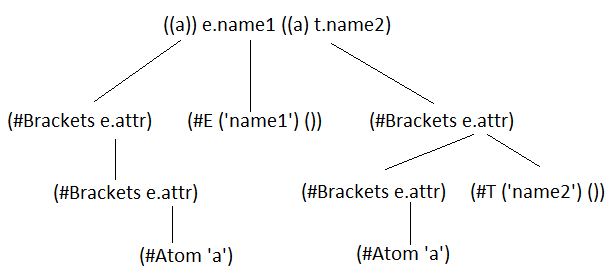
\includegraphics[width=0.7\linewidth]{./chapter3/tree}
\caption{Пример синтаксического дерева}
\label{fig:tree}
\end{figure}


\subsection[Обобщение образцов]{\large Обобщение образцов}
\subsubsection[Генерация жестких образцов]{\large Генерация жестких образцов}
\hspace{\parindent} Как говорилось в пункте \ref{sec:optimization}, на первом этапе оптимизации все образцы функции приводятся к жестким образцам. Алгоритм получения СЖО описан в пункте \ref{sec:sjo}. Для того что бы не <<протаскивать>> между вызовами счётчик, инкрементируемый для каждой переменной, ее новое имя представляется уникальной  последовательностью букв 'l', 'c', и 'r'. Функция генерации индексов принимает на вход образец, разбитый на лексемы и последним аргументом в структурных скобках --- текущий индекс. Если образец можно разбить таким образом:
\begin{equation*}
\begin{array}{l}
\textrm{e.smth1 ( e.smth2 ) e.smth3} \\
\end{array}
\end{equation*}
\indent то для каждой из частей происходит рекурсивный вызов функции генерации индексов со следующими добавлениями к текущему индексу
\begin{equation*}
\begin{array}{l}
\textrm{e.smth1 - текущий индекс + 'l' - спуск в левую часть} \\
\textrm{e.smth2 - текущий индекс + 'c' - спуск <<по центру>>} \\
\textrm{e.smth3 - текущий индекс + 'r' - спуск в правую часть} \\
\end{array}
\end{equation*}

\indent Если скобок нет, то отщипывается терм слева, а для оставшейся правой части опять происходит рекурсивный вызов, с добавлением буквы 'r' к текущему индексу. Если <<оторванный>> терм - переменная, то ее имя меняется на текущий индекс + 'l'. \\ \indent В примере \ref{eq:sjo_examplik} показано, как будет выглядеть СЖО для образца с открытыми и повторными переменными.

\begin{equation}\label{eq:sjo_examplik}
\begin{array}{l}
\textrm{Образец: (t.1) e.1 () e.2 () e.1} \\
\textrm{Жесткий образец: (t.Index\_l) e.Index\_r} \\
\textrm{Подстановка для t.Index\_l} \rightarrow \textrm{[t.1]} \\
\textrm{Подстановка для e.Index\_r} \rightarrow \textrm{[e.1 () e.2 () e.1]} \\
\end{array}
\end{equation}

\subsubsection[Быстрое обобщение]{\large Быстрое обобщение}
\hspace{\parindent} ...
\subsubsection[Глобальное сложнейшее обобщение]{\large Глобальное сложнейшее обобщение}
\hspace{\parindent} ...

\clearpage
\newpage

\part*{\large \centering ЗАКЛЮЧЕНИЕ}
\addcontentsline{toc}{part}{ЗАКЛЮЧЕНИЕ}
\hspace{\parindent}

\clearpage
\newpage
\bibliographystyle{utf8gost705u}  %% стилевой файл для оформления по ГОСТу
\begin{flushleft}
\bibliography{biblio}     %% имя библиографической базы (bib-файла) 
\end{flushleft}

\end{document}
